\scanpage{137}
\begin{center}- 37 -\end{center}
\margin{n°338}
\uline{l'homomorphisme} $x\longrightarrow1\otimes x$ \uline{de} $F$ \uline{dans} $B\otimes_A F$ \uline{est injectif} ;

(iv) \uline{le} $A$-\uline{module à droite} $B$ \uline{est plat, et, pour tout idéal à gauche} $\underline a$ \uline{de} $A$ \uline{on a} $h^{-1}(B\underline a)=\underline a$.

(v) \uline{le} $A$-\uline{module à droite} $B$ \uline{est plat, et, pour tout idéal à gauche maximal} $\underline m$ \uline{de} $A$, \uline{il existe un idéal à gauche maximal} $\underline{m'}$ \uline{de} $B$ \uline{tel que} $h^{-1}(\underline{m'})=\underline m$.
\margin{$\unsure{\operatorname{Spec}|\operatorname{Spm}}(B)\longrightarrow\unsure{\operatorname{Spec}|\operatorname{Spm}}(A)$ surjectif}
\figure{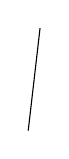
\begin{tikzpicture}\draw(0,0)--(.15,1.3);\end{tikzpicture}}

En effet, d'après le lemme, (i) implique chacune des propriétés (iii), (iv), (v). D'autre part, si (v) est vérifiée, on a $B\underline m\ne B$ pour tout idéal à gauche maximal $\underline m$ de $A$, et $B$ est fidèlement plat sur $A$ par définition.

Nous allons maintenant prouver que $(i)\Longrightarrow(iii)\Longrightarrow(iv)\Longrightarrow(ii)\Longrightarrow(i)$, ce qui achèvera la démonstration. On a déjà vu que (i) implique (iii). D'autre part (iii) implique (iv) en prenant $F=A/\underline a$. Si (iv) est vérifié, on voit, en prenant $\underline a=(0)$, que $h$ est injectif, et on a la suite exacte
\diagram{\begin{tikzcd}
0\arrow[r]&A\arrow[r,"h"]&B\arrow[r]&B\,h(A)\arrow[r]&0\,;
\end{tikzcd}}
cette suite vérifie la condition c) de la prop.3 du § 2 (cf. la remarque suivant cette proposition) ; d'après ladite proposition, il s'ensuit que $B/h(A)$ est plat, d'où (ii). Enfin, si (ii) est vérifiée, la prop. 3 appliquée à la suite exacte $0\longrightarrow A\xrightarrow{h}B\longrightarrow B/h(A)\longrightarrow0$ montre que $B$ est fidèlement plat. CQFD.

Dans les conditions de la prop.8, identifions $A$ à un \uline{sous-anneau} de $B$ au moyen de $h$. La relation (iv) s'écrit alors $A\cap B\underline a=\underline a$ pour tout idéal à gauche $\underline a$ de $A$. D'autre part, si $F$ est un $A$-module à gauche, on identifie $F$ à son image dans $B\otimes_A F$ par l'application $x\longrightarrow1\otimes x$ ; si $X$ est un sous-groupe additif de $F$, on note alors $BX$ le sous-$B$-module à gauche de $B\otimes_A F$ engendré par $X$. Avec ces notations on a :

PROPOSITION 9.- \uline{Soient} $B$ \uline{un anneau et} $A$ \uline{un sous-anneau de} $B$ \uline{tels que} $B$ \uline{soit}
\mspage{136}

